
\documentclass[11pt]{article}
\usepackage{graphicx}
\graphicspath{{./Images/}}
\usepackage{setspace}
\usepackage{subcaption}
\usepackage{multirow}
\usepackage{diagbox}
\usepackage{color, colortbl}
\definecolor{yellow}{rgb}{1,1,0.25}
\usepackage[left=3.2cm, right=3.2cm, top=3cm]
{geometry}
\setstretch{1.5}
\usepackage[bottom]{footmisc}
\begin{document}
\title{Predicting NBA Regular Season Results Based on some popular statistics}
\author{Chenjie Li, Qiao Qiao, Giyoon Kwag}
\maketitle

\vspace*{3\baselineskip}
\begin{center}
Contributions:\\
\end{center}
\begin{center}
\begin{tabular}{|c|c|c|c|}
\hline
Name & Chenjie Li& Qiao Qiao & Giyoon Kwag\\
\hline
Contribution &  $33.33\%$ & $33.33\%$ & $33.33\%$ \\
\hline
\end{tabular}
\end{center}
\newpage

\section*{1.Problem Description}
\subsection*{1.1 Background}
\hspace{1.5em} NBA (National Basketball Association) is one of the most successful basketball league around the world.And since it is popular, there exists tons of websites recording the statistics related to the game. They not only provide simple metrics like Field Goal Percentage,  Average Points, Average Assists, but also some advanced metrics like PER,True shooting percentage and much more.

Based on those statistics, people have been exploring what kinds of metrics can result in a team's success or failure as a season, or what metrics or combination of different metrics can result in team's success.

In this report, we investigated the relationship between the regular season results of the team and some popular metrics in two different perspectives: 
\begin{itemize}
\item \textbf{Teams' Overall Effects}: \textbf{Team's Offensive Efficiency (TOE)}
\item \textbf{Teams' Net Rating}
\end{itemize}
From those 3 metrics above, we proposed new TOE and NEW Teams' Net Rating and compared models by using ``Cross Validation method", we found out that our new version of those two metrics are stronger correlated with teams' win ratios than the results for old versions.
In this report, we collected data for the past 5 seasons ($2014-2018$).Based on the results we get from 2014-2017 seasons, we made some predictions for the results of this 2018 season and compare the results between our predictions and the real results.

\section*{2.Data Source}
\hspace{1.5em} There are many ``data hubs" available, our data source is mainly from \\insider.espn.com/nba/hollinger/statistics ,https://www.basketball-reference.com/ and\\ http://www.espn.com/nba/statistics

To be able to work with data, we deveoped a ``web crawler" using Python ``Scrapy" module. By using the program we got the formatted CSV file so that we can easily input them in R.

Furthermore, since we are familiar with Database and SQL language, we also put the data in a database so we can manipulate the data easily by Queries.
\section*{3.Win Ratio Analysis}
\subsection*{3.1 New TOE introduction and Experiments}
\hspace{1.5em}Offensive Efficiency, as the name suggests, is a parameter measuring the efficiency of the offense. Here we explain this intuition by giving an example:

Player A took 5 shots and made 4 of them; Player B took 5 five shots, and made 2 of them. Therefore, we can conlcude that player A is more efficient than Player B.

Of course, this is a oversimplified example.

There are a lot different kinds of definitions for Player and Team's Efficiency:
In Shea,Stephen M's book$^{[1]}$, They define the Offensive Efficiency for Team as:
\begin{center}
$TOE = \frac{FG}{FGA \;-\; ORB\; + \;TO}$
\end{center}

Where FG is the field goals made, FGA is the field goals attempts, ORB is the number of offensive rebounds, TO represents the number of turnovers. 

It is of course reasonable to guess that the more efficient a team's offensive is, the more number of games a team is going to win.This idea was proved in their book: ``The top 5 teams in TOE in the 2012-2013 season all won at least 56 games."

This book was written and published five years ago. As time goes by, NBA statistics has been getting more and more comprehensive.
Now we want to propose a new version of Team's offensive efficiency.

The formula we proposed is:
\begin{center}
$New\;TOE = \frac{2PTM \;+ \;1.5 \;* \;3PTM}{FGA \;-\; ORB \;*\; ORBS \; + \;TO\; * \;OPPOTS}$
\end{center}
Where \textit{2PTM}means 2 points field goals made;\textit{3PTM} means 3 points field goals made; \textit{ORBS} means the offensie rebound scoring rate; \textit{OPPOTS} means opponent scoring rate off the team's turnovers.

Now let's motivate our formula. An individual offensive possesion could lead up to 4 possible results: taking a 2 point shot, taking a 3 point shot, missing a shot but getting an offensive rebound, and turning the ball over. We assume that a 3 point shot made is 1.5 times as great as a 2 point shot made. Offensive rebound could compensate the results of missing the shot.Since most(not all of them, of course) second chance points are 2 points, we ignored the effect of the 3 point second chance points.but here we times Offensive rebound by ``offensive rebound scoring rate", because different teams might have different abilities to convert a offensive rebound to box score.Here we also ignored the effect of 3 points made by opponent off turnovers.And finally, we add a factor ``$TO\; * \;OP\_POTS\%$" to take the effects of turnovers into consideration.

In this section all our data is from \textit{https://stats.nba.com/}$^{[2]}$.

We calculated the results from Season 2014 - Season 2017, here we only show two groups of results. For comprehensive results, please check out the Appendix part.
\begin{figure}[h!]
  \centering
  \begin{subfigure}[b]{0.45\linewidth}
    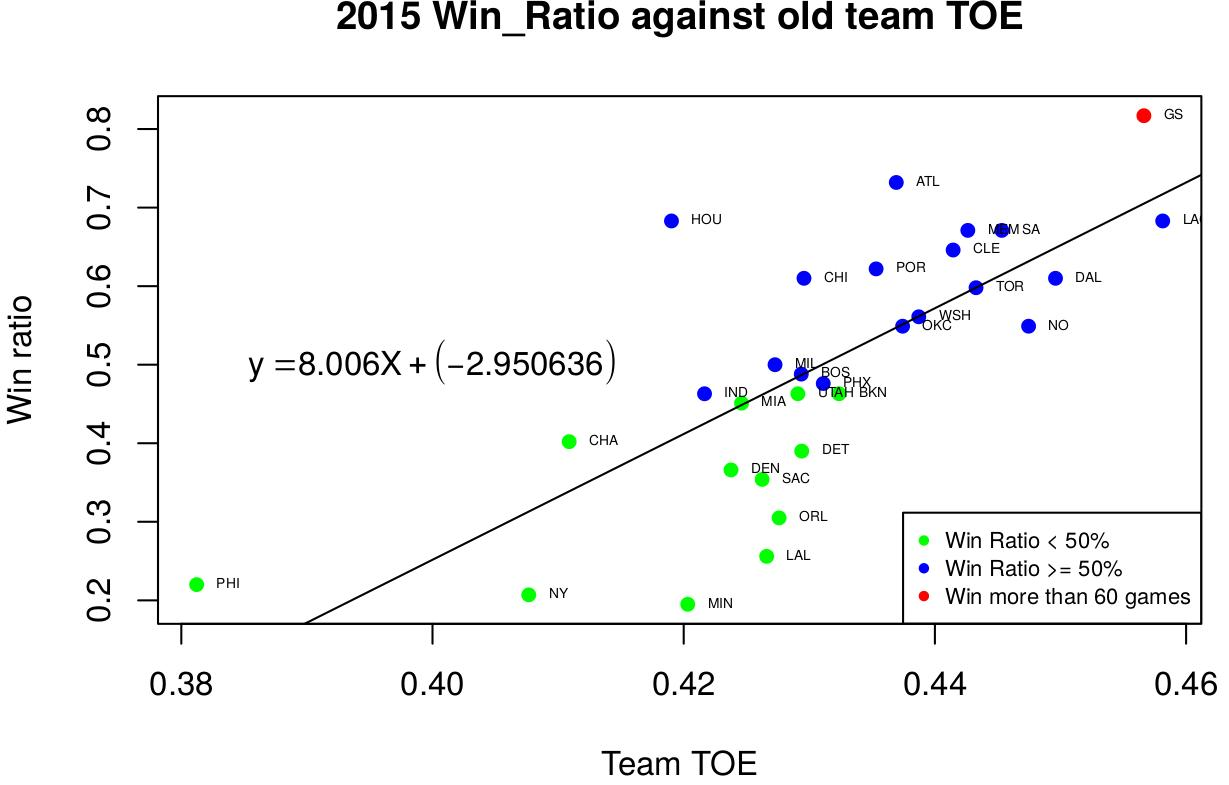
\includegraphics[width=\linewidth]{15old.jpg}
  \end{subfigure}
      \caption{2015 Season Using Old TOE}
  \begin{subfigure}[b]{0.45\linewidth}
    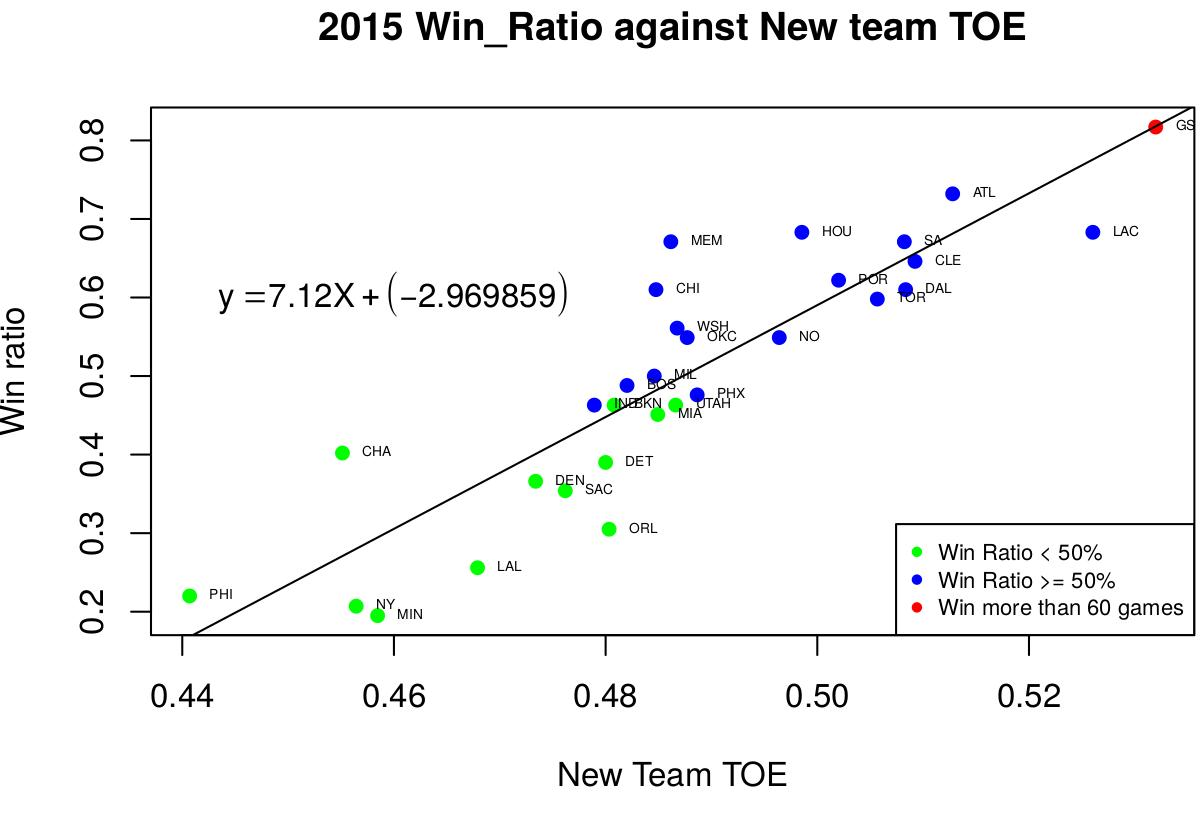
\includegraphics[width=\linewidth]{15new.jpg}
  \end{subfigure}
    \caption{2015 Season Using New TOE}

\end{figure}
\begin{figure}[h!]
\centering
 \begin{subfigure}[b]{0.4\linewidth}
  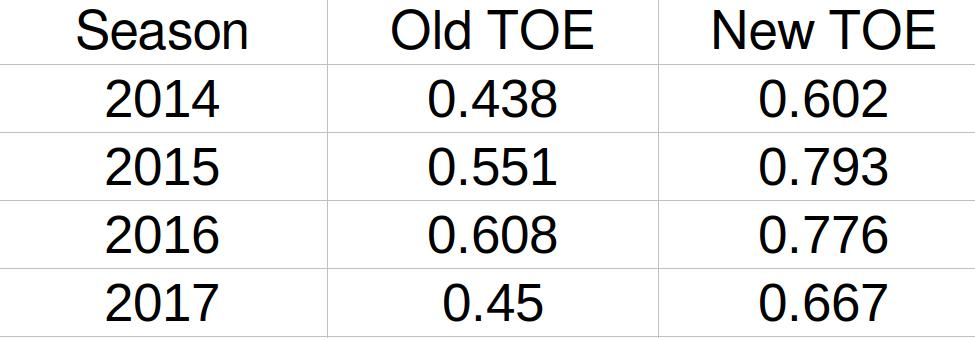
\includegraphics[width=\linewidth]{ComparisionR.jpg}
 \end{subfigure}
 \begin{subfigure}[b]{0.4\linewidth}
  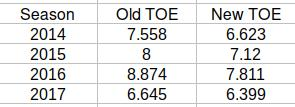
\includegraphics[width =\linewidth]{Beta1.jpg}
\end{subfigure}
 \caption{Comparison of $R^2$(left) and $\beta_1$(right)}
\end{figure}

As Figure 1 and Figure 2 show, our new TOE is much better(significantly higher $R^2$ value) than evaluating the relationship between Win Ratio and Team Offensive Efficiency. We noticed the coefficient $\beta_1$ values keep increasing in 3 consectutive years, whereas in 2017 the $\beta_1$
drops again.

\newpage
\subsection*{3.2 Module comparison and validation}
\subsubsection*{Train Test and AIC$_p$}
Now we pay our attention to the evaluation of the model.
In this section we use ``Correlation Accuracy". A simple correlation between the actuals and predicted values can be used as a form of accuracy measure. A higher correlation accuracy implies that the actuals and predicted values have similar directional movement, i.e. when the actuals values increase the predicteds also increase and viceversa$^{[3]}$.

Also, we calculated AIC$_p$,Akaike information criterion$^{[4]}$ to compare between old model and the new model.

\begin{center}
\begin{tabular}{|c|c|c|c|}
\hline
Statistic & Train:Test Ratio& Old TOE & New TOE\\
\hline
Train,Test Score & 5:1 & 0.757 & 0.810\\
Train,Test Score & 4:1 & 0.757 & 0.812\\ 
Train,Test Score & 3:1 & 0.754 & 0.825\\ 
\hline
Train,Test Score & Avgerage& 0.757 & 0.816\\
\hline 
AIC$_P$& 5:1 & -152.2682 & -186.1824 \\
AIC$_P$& 4:1 & -145.4626 & -178.7008 \\
AIC$_P$& 3:1 & -138.7349 & -166.051 \\
\hline
AIC$_P$& Average & -136.489 & -176.978 \\
\hline
\end{tabular}

\bigskip
Table 1: Tran Test Accuracy And AIC$_p$
\end{center}
From Table 1 we could clearly see that our new TOE has better correlation accuracy and smaller AIC$_p$ values.

\subsubsection*{K-Fold Cross Validation}
In this section, we compare the module performances by using 
Cross Validation, which, in essense, is just a systematic evaluation by implementing ``train and test" procedure.
We splitted our data into `k' mutually exclusive random sample portions. Each time, we keep one of the portions as test data, we build the model on the remaining (k-1 portion) data and calculate the mean squared error of the predictions. This is done for each k random samples.
In this report, we chose K = 5 and K = 4 as our ``fold number", which means we divided our data(120 points) into 5 and 4 groups, respectively.

The results are shown below:

\begin{center}
\begin{tabular}{|c|c|c|}
\hline
 K value & Old Toe & New Toe \\
\hline
 4 & 0.45 $\pm$ 0.18 & 0.50 $\pm$ 0.23\\
 5 & 0.47 $\pm$ 0.12 & 0.51 $\pm$ 0.27 \\
\hline
\end{tabular}
\bigskip

Table 2:Correlation Accuracy( $\pm 95\%$CI) for Old TOE and New TOE
\end{center}

\subsection*{3.3 Prediction And Evaluation}
After model validation procedures, we believe that our proposed new model has stronger correlations with win ratios.
Now it's time to see the prediction results for 2018 seasons.

The Results are shown below:

\begin{figure}[h!]
  \centering
  \begin{subfigure}[b]{0.45\linewidth}
    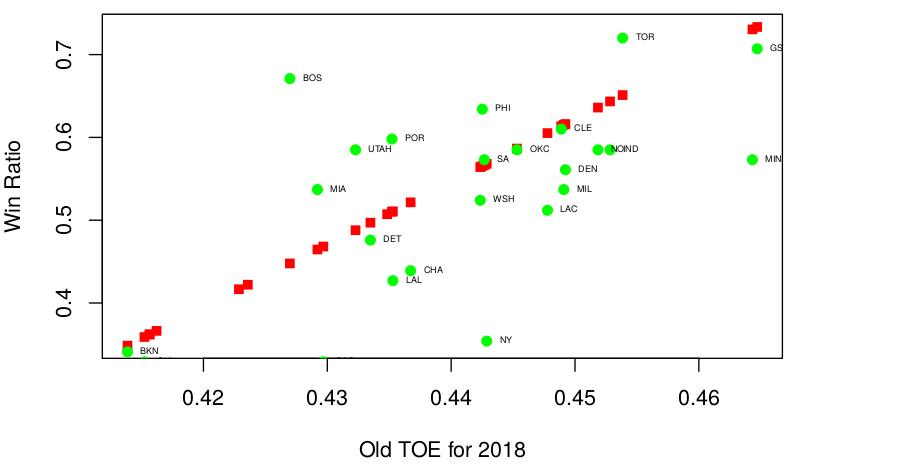
\includegraphics[width=\linewidth]{old_toe.jpg}
  \end{subfigure}
  \begin{subfigure}[b]{0.45\linewidth}
    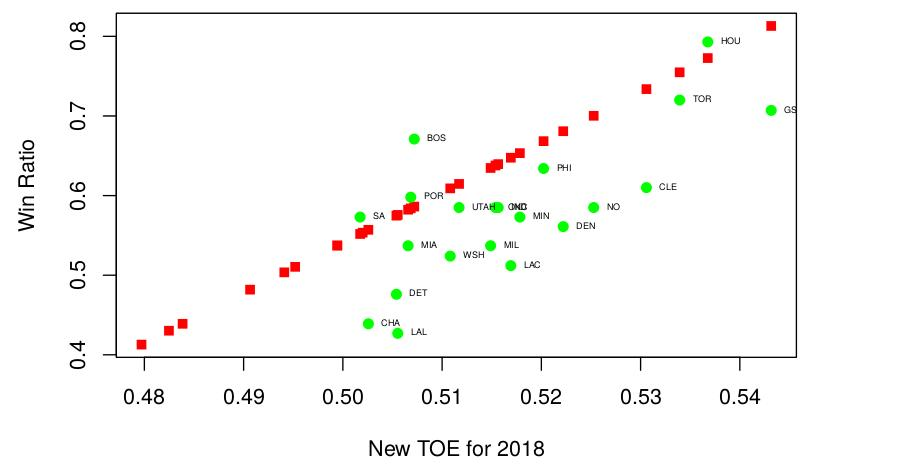
\includegraphics[width=\linewidth]{new_toe_pred.jpg}
  \end{subfigure}
  \caption{Predictions for 2018 season( left:Old TOE, right: New TOE)}
\end{figure}
From the results above, we calculated Sum of square errors for both of the model. $SSE_{old}$ = 0.35, $SSE_{new}$ = 0.474.

The results we got surprisingly contradict our expectations. 
Despite those results,we believe our model is still better than the old model in the following reasons:
\begin{itemize}
\item In the previous section, every metric evaluation or validation result show that our proposed model is a better fit.
\item If we see the prediction graph in detail, we can clearly see in the result of our proposed model, there definitely exists strong correlation between win ratio and new TOE.We believe 2018 is an unique season during which almost all of the teams ``quality" of the offense were ``weakend".
\end{itemize}
\section*{4. Net Rating}
\subsection*{4.1 Net Rating Definition}
In the previous section, our prediction results were inaccurate because of the ``weakened" quality of offensive efficiency.In this section, we introduce the Opponent Team Offensive Efficiency into our ``Net Rating" metric and do the same evaluation procedures (Evaluation,Validation,Prediction).
The most likely ``factor" resulting in this unexpected result is because of today's NBA trend: Most Teams in the league are paying more attention on their offense, whereas they are ignoring the importance of the defense.
First, let's define Net Rating:\\

In this Net Rating definition, we added what is missing in TOE part: The opponents' effect.\\
Net Rating:
\begin{center}
$100*(\frac{FGM}{FGA\;-\;ORB\;*\;+\;TO}\;-\;\frac{OPFGM}{OPFGA\;-\;OPORB\;+\;OPTO})$\\
\end{center}
Where:
\begin{center}
OPTOE = $\frac{OPFGM}{OPFGA\;-\;OPORB\;+\;OPTO}$\\
\end{center}
New Net Rating:
\begin{center}
$100*(\frac{2FGM\;+\;1.5\;*\;3FGM}{FGA\;-\;ORB\;*\;ORBS\;+\;TO*OPPOTS}\;-\;\frac{OP2FGM\;+\;1.5\;*\;OP3FGM}{OPFGA\;-\;OPORB\;*\;OPORBS\;+\;OPTO\;*\;POTS})$\\
\end{center}
Where:\\
\begin{center}
$New\;OPTOE = \frac{OP2FGM\;+\;1.5\;*\;OP3FGM}{OPFGA\;-\;OPORB\;*
\;OPORBS\;+\;OPTO\;*\;POTS}$\\
\end{center}

Just as what we've defined in TOE and New TOE, we added opponents' performance.OP2FGM is a team's opponents' average 2 point field goals made per gam. OP3PM is a team's opponents' average 3 point field goals made per game; OPFGA is a team's opponents' average field goal attempts; OPORB is a team's opponents' average offensive rebound; OPORBS is a team's opponents' ``offensive rebound scoring rate" against this team being evaluated; OPTO is a team's opponents' average turnovers; and at last, POTS the team's scoring rate off the opponents' average turnovers.

After subtraction operation, we times the resulst by 100, so this means \textbf{this team's net win margin in 100 possessions}

\subsection*{4.2 Experiments}
As Section 3 for TOEs, we also tested our Net Ratings on 2014-2017 seasons.
The results for 2015 season are shown below, for comprehensive results, please check out the Appendix part.

\begin{figure}[h!]
  \centering
  \begin{subfigure}[b]{0.45\linewidth}
    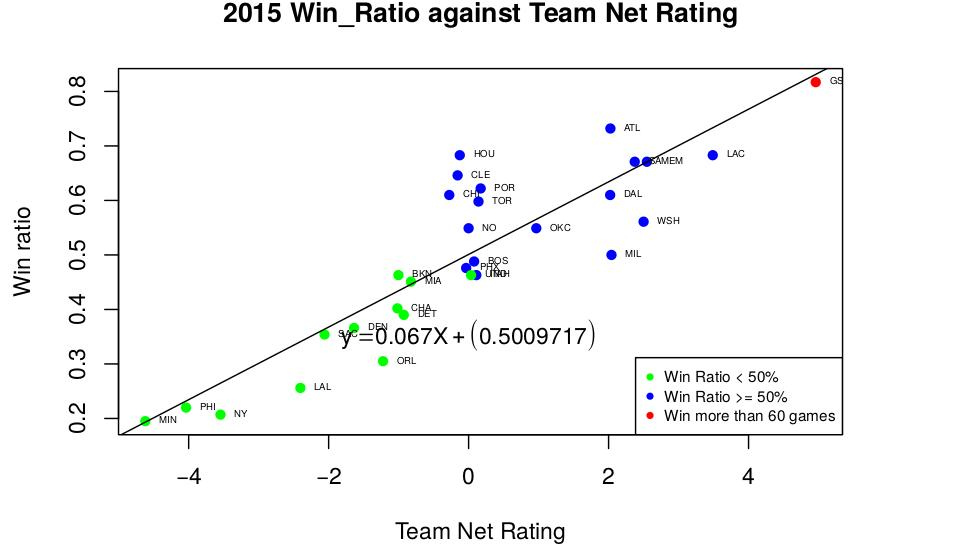
\includegraphics[width=\linewidth]{old_nr.jpg}
  \end{subfigure}
  \caption{2015 Season Using Net Rating}
  \begin{subfigure}[b]{0.45\linewidth}
    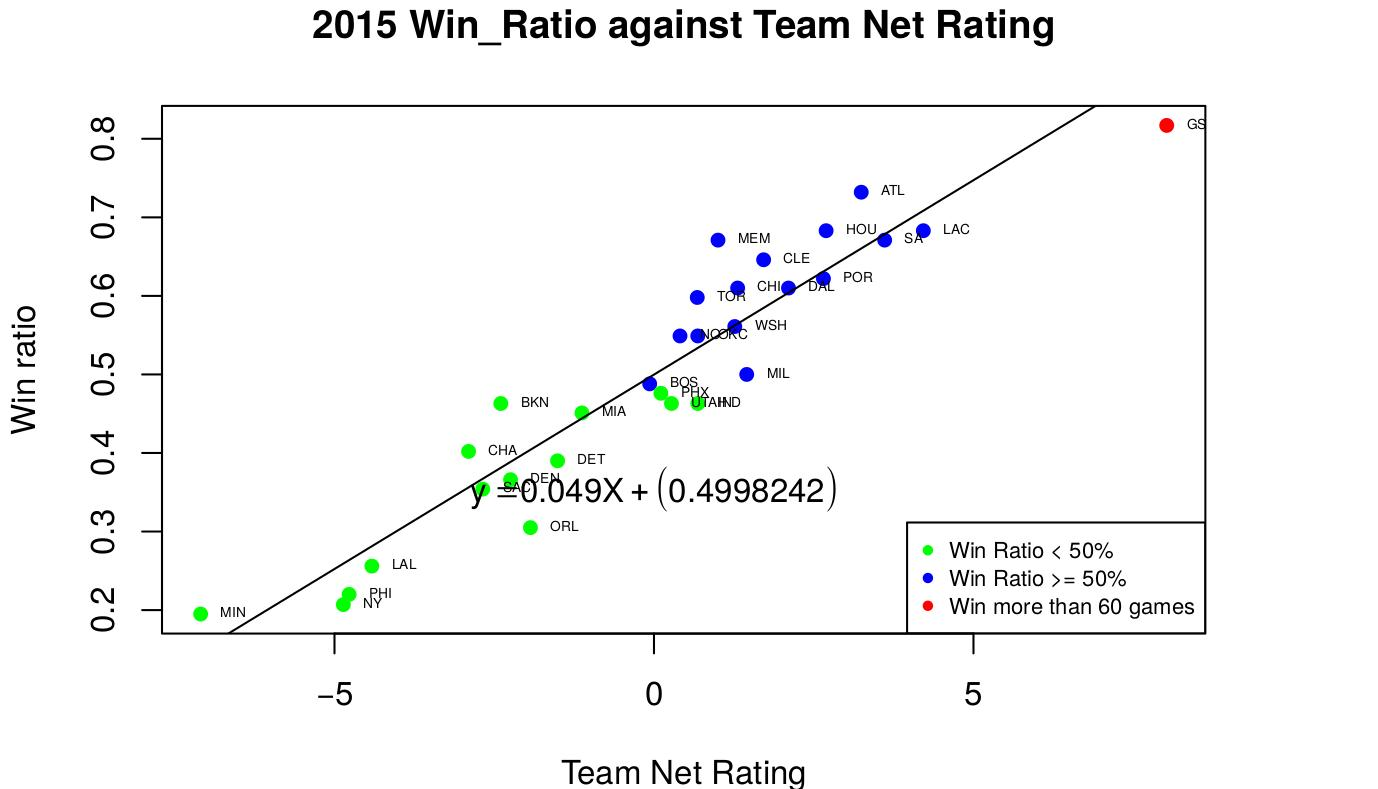
\includegraphics[width=\linewidth]{new_nr.jpg}
  \end{subfigure}
    \caption{2015 Season Using New Net Rating}
\end{figure}

\begin{center}
\begin{tabular}{|c|c|c|c|c|c|}
\hline
Season& Net Rating $R^2$ & New Net Rating $R^2$ & Season& Net Rating $\beta_1$ & New Net Rating $\beta_1$\\
\hline
 2014& 0.784 & 0.895 &2014 & 0.065 & 0.052 \\
 2015& 0.776 & 0.895 &2015 & 0.067 & 0.049 \\ 
 2016& 0.822 & 0.882 &2016 & 0.064 & 0.048 \\
 2017& 0.699 & 0.838 &2017 & 0.061 & 0.048 \\
\hline
\end{tabular}
\bigskip

Table 3: Comparison of $R^2$(left) and $\beta_1$(right) for Net Ratings
\end{center}

As Figure 4 and Table 3 show, our New Net Rating is better (higher $R^2$ value) than evaluating the relationship between Win Ratio and Team Offensive Efficiency.One thing we noticed is that $\beta_1$ and $R^2$ are all very steady across those 4 years.

\newpage
\subsection*{4.3 Module comparison and validation}
\subsubsection*{Train Test and AIC$_p$}
Just as what we did for TOEs, we also evaluated thos two different Net Ratings using 
AIC$_p$, Train Test and K-Fold Cross validation.
\begin{center}
\begin{tabular}{|c|c|c|c|}
\hline
Statistic&Train:Test Ratio& Net Rating & New Net Rating\\
\hline
Train,Test Score & 5:1 & 0.885 & 0.965 \\
Train,Test Score & 4:1 & 0.888 & 0.962\\ 
Train,Test Score & 3:1 & 0.891 & 0.956 \\ 
\hline
Train,Test Score & Avgerage& 0.888 & 0.961\\
\hline 
AIC$_P$& 5:1 & -235.3074 & -289.7162\\
AIC$_P$& 4:1 & -225.8254 & -279.0621\\
AIC$_P$& 3:1 & -212.9546 & -261.1197 \\
\hline
AIC$_P$& Average & -224.6958 & -276.6327\\
\hline
\end{tabular}

\bigskip
Table 4: Tran Test Accuracy And AIC$_p$
\end{center}
From Table 1 we could clearly see that our new Net Rating has better correlation accuracy and smaller AIC$_p$ values than those of Net Rating.

\subsubsection*{K-Fold Cross Validation}
In this section, we compare the module performances by using 

The results are shown below:

\begin{center}
\begin{tabular}{|c|c|c|}
\hline
 K value & Net Rating & New Net Rating \\
\hline
 4 & 0.74 $\pm$ 0.12 & 0.86 $\pm$ 0.06\\
 5 & 0.75 $\pm$ 0.12 & 0.86 $\pm$ 0.07 \\
\hline
\end{tabular}
\bigskip

Table 5:Correlation Accuracy( $\pm 95\%$CI) for Net Rating and New Net Rating
\end{center}

\subsection*{4.4 Prediction And Evaluation}

Now it's time to see the prediction results for 2018 seasons.

The Results are shown below:

\begin{figure}[h!]
  \centering
    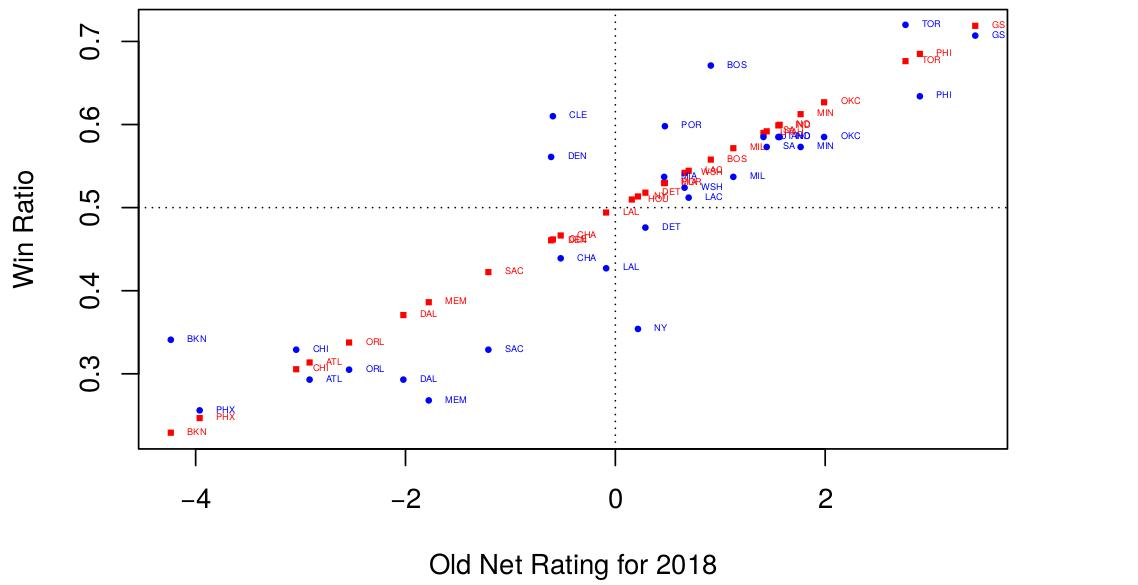
\includegraphics[width=\linewidth]{old_nr_pre.jpg}
  \caption{Predictions for 2018 season using Net Rating}
\end{figure}

\begin{figure}[h!]
  \centering
    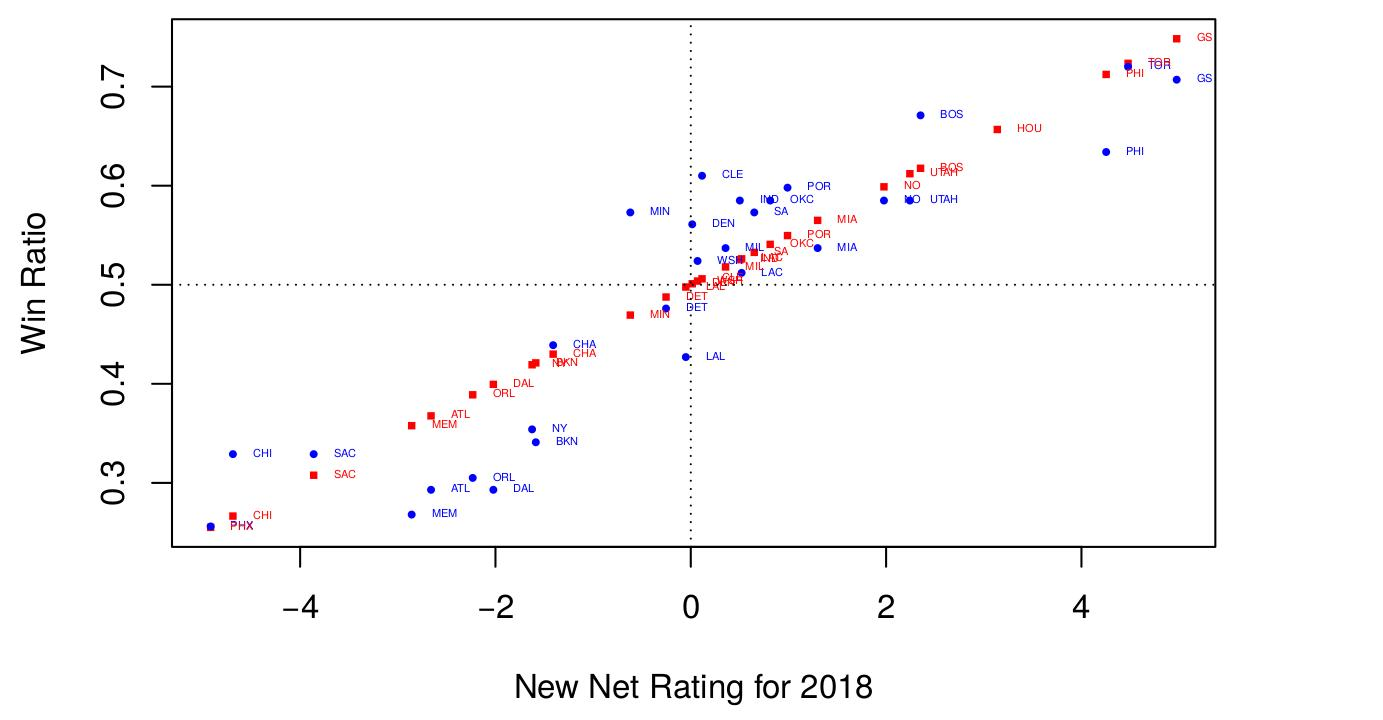
\includegraphics[width=\linewidth]{new_nr_pre.jpg}
  \caption{Predictions for 2018 season using Net Rating}
\end{figure}

From the results above, we calculated sum of squares for both of the model. $SSE_{old}$ = 0.217, $SSE_{new}$ = 0.119.

Here are the comparison between two versions of Net Ratings and the Real Results:\\

\begin{center}
\begin{tabular}{|c|c|c|c|c|c|c|c|}
\hline
\multicolumn{4}{|c|}{New Net Rating} &
\multicolumn{4}{c|}{Net Rating} \\
\hline
\multicolumn{2}{|c|}{Western Conference} &
\multicolumn{2}{c|}{Eastern Conference}&
\multicolumn{2}{c|}{Western Conference} &
\multicolumn{2}{c|}{Eastern Conference}\\

\hline
 Team& Win Ratio & Team & Win Ratio & Team & Win Ratio &Team & Win Ratio \\
\hline
\cellcolor{yellow} GS   & 0.748 & \cellcolor{yellow} TOR & 0.724 & \cellcolor{yellow} GS   & 0.719 & \cellcolor{yellow} PHI & 0.685\\
\hline
\cellcolor{yellow} HOU  & 0.657 & \cellcolor{yellow} PHI & 0.712 & \cellcolor{yellow} OKC  & 0.627 & \cellcolor{yellow} TOR & 0.676 \\
\hline
\cellcolor{yellow} UTAH & 0.612 & \cellcolor{yellow} BOS & 0.618 & \cellcolor{yellow} MIN  & 0.612 & \cellcolor{yellow} IND & 0.599\\
\hline
\cellcolor{yellow} NO   & 0.599 & \cellcolor{yellow} MIA & 0.565 & \cellcolor{yellow} NO   & 0.600 & \cellcolor{yellow} MIL & 0.572\\
\hline
\cellcolor{yellow} POR  & 0.550 & \cellcolor{yellow} IND & 0.525 & \cellcolor{yellow} SA   &  0.592 & \cellcolor{yellow} BOS & 0.558 \\
\hline
\cellcolor{yellow} OKC  & 0.541 & \cellcolor{yellow} MIL & 0.518 & \cellcolor{yellow} UTAH & 0.590 & \cellcolor{yellow} WSH & 0.542 \\
\hline
\cellcolor{yellow} SA   & 0.533 & \cellcolor{yellow} CLE & 0.506 & LAC &  0.544 & \cellcolor{yellow} MIA & 0.529\\
\hline
 LAC  & 0.526 & \cellcolor{yellow}  WSH & 0.504 &  \cellcolor{yellow} POR &  0.530 & DET & 0.518\\
\hline
\end{tabular}

\bigskip

Table 6: 2018 End Of Season Playoffs Prediction \\(Yellow means correct prediction if this team is in the first 8 seeds in its conference)
\end{center}


\begin{center}
\begin{tabular}{|c|c|c|c|}
\hline
\multicolumn{4}{|c|}{2018 Playoffs Standings(Actual Results)}\\
\hline
\multicolumn{2}{|c|}{Western Conference} &
\multicolumn{2}{c|}{Eastern Conference} \\
\hline
Team& Win Ratio & Team & Win Ratio \\
\hline
HOU  & 0.793 & TOR & 0.720\\
\hline
GS   & 0.707 & BOS & 0.671\\
\hline
POR  & 0.598 & PHI & 0.634\\
\hline
OKC  & 0.585 & CLE & 0.610\\
\hline
UTAH & 0.585 & IND & 0.585\\
\hline
NO   & 0.585 & MIA & 0.537\\
\hline
SA   & 0.573 & MIL & 0.537\\
\hline
MIN  & 0.573 & WSH & 0.524\\
\hline
\end{tabular}
\bigskip

Table 7: The Actual Playoffs Rankings
\end{center}

\newpage
\subsection*{4.5 Analysis And Conclusion}

From the results shown above, we can clearly see that the prediction is very accurate in terms of ``who make the playoffs", except some exceptions:\\
Houston Rockets, who was actually top seed in Western Conference, in ``Net Rating Mdel", are surprisingly left out from the Playoffs, whereas in ``New Net Rating" model, Houston ranked in the second seed.\\
Another surprise is Lebron James' Cavs team, which ranked 4th at the end of last regular season, are both ranked very low in our two models(7th in New Net Rating Model,11th in the Net Rating Model). I think Lebron is really someone special who can turn things around.\\

In terms of win ratio predictions, New Net Rating Model has 

\begin{center}
\begin{tabular}{|c|c|c|c|}
\hline
\backslashbox{Win Ratio}{Category}
& New Net Rating & Net Rating & Actual Results\\
\hline
Team& Win Ratio & Team & Win Ratio \\
\hline
$\geq 0.7$ & 3 & 1 & 3 \\
\hline
$\geq 0.6$ & 3 & 5 & 3\\
\hline
$\geq 0.5$ & 10 & 10 & 10 \\
\hline
\end{tabular}
\bigskip

Table 8: Distribution of Teams in terms of Win Ratio
\end{center}
From the table shown above, we can clearly see that our New Net Rating model has exactly same number of teams in different win ratio ranges.

\newpage
\section*{5. Conclusions}

In this report, we proposed modified models, New TOE and New Net Rating, and for each new model we made some predictions using past 4 years data and did some model validations and model comparisons.

The results show when evaluating the models to predict NBA regular season results, both teams' offense and defense should be considered so that we can make more accurate predictions.

\section*{References}
1. Shea, S. M., Baker, C. E. (2013). Basketball analytics: Objective and efficient strategies for understanding how teams win. CreateSpace Independent Pub. Platform.\\
2. Teams General Misc Statistics. Retrieved from \textit{stats.nba.com} \\
3. Simple linear regression: A complete introduction with numeric example, Retrieved from \textit{http://rstatistics.net/linear-regression-with-r-a-numeric-example/}\\
4. Neter, J., Kutner, M. H., Nachtsheim, C. J.,  Wasserman, W. (1996). Applied linear statistical models (Vol. 4, p. 359). Chicago: Irwin.


\newpage
\section*{6. Appendix}

\subsection*{\S \hspace{0.8em} \textbf{Glossary}}
\textbf{TOE}:Teams Offensive Efficiency\\
\textbf{FG}: Field Goals Made\\
\textbf{FGA}: Field Goal Attempts\\
\textbf{ORB}: Offensive Rebounds\\
\textbf{TO}: Turnovers\\
\textbf{2PTM}: 2 Points Total Made\\
\textbf{3PTM}: 3 Points Total Made\\
\textbf{ORBS}: Offensive Rebound Scoring Rate\\
\textbf{OPPOTS}: Opponent Points Scored Off Team' s Turnovers Scoring Rate\\
\textbf{OPFGA}: Opponent Field Goal Attempt\\
\textbf{OPORB}: Opponent Offensive Rebound\\
\textbf{OPTO}: Opponent Turnovers\\
\textbf{OPTOE}: Opponent Team Offensive Efficiency\\
\textbf{OP2FGM}: Opponent 2 Points Field Goals Made\\
\textbf{OPORBS}: Opponent Offensive Rebound Scoring Rate\\
\textbf{POTS}: Points Off Scored Off Opponent Team's Turnovers Scoring Rate\\

\newpage

\newpage
\subsection*{\S Results of The Other Years}

\subsubsection*{Net Ratings from 2014-2017 Seasons}
\begin{figure}[h!]
  \centering
  \begin{subfigure}[b]{0.45\linewidth}
    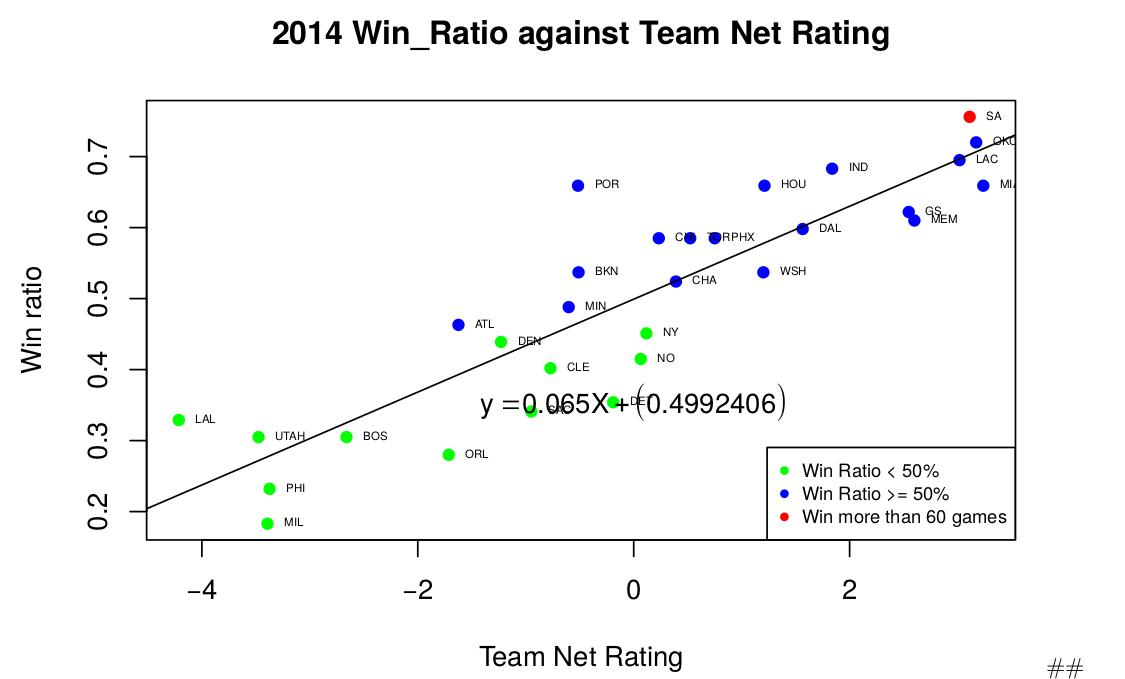
\includegraphics[width=\linewidth]{nr_14.jpg}
  \end{subfigure}
  \begin{subfigure}[b]{0.45\linewidth}
    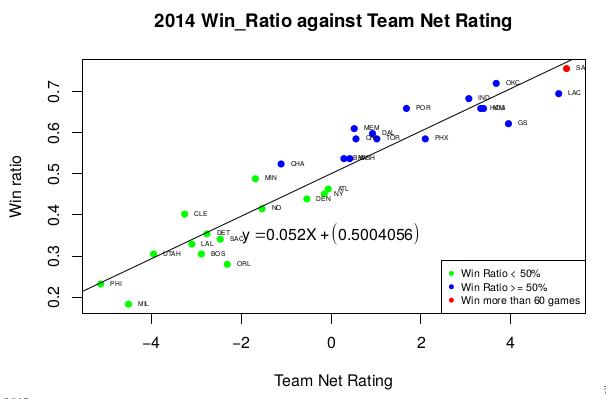
\includegraphics[width=\linewidth]{new_nr_14.jpg}
  \end{subfigure}

\bigskip
Figure 1: Comparison Between Net Rating and New Net Rating in 2014 Season
\end{figure}

\begin{figure}[h!]
  \centering
  \begin{subfigure}[b]{0.45\linewidth}
    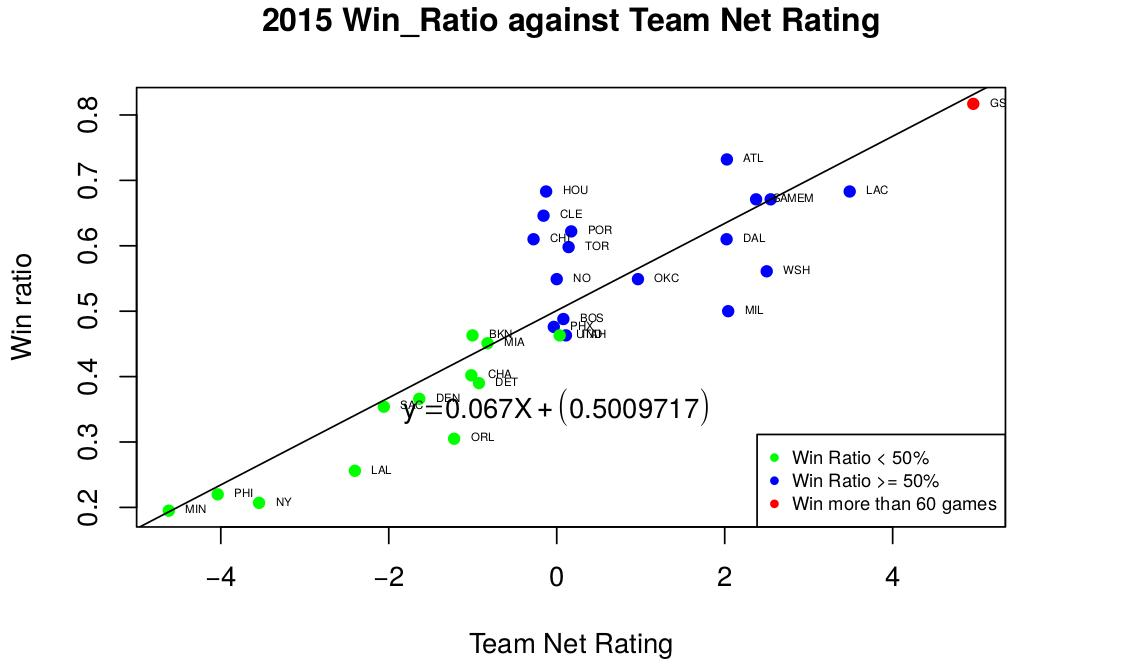
\includegraphics[width=\linewidth]{nr_15.jpg}
  \end{subfigure}
  \begin{subfigure}[b]{0.45\linewidth}
    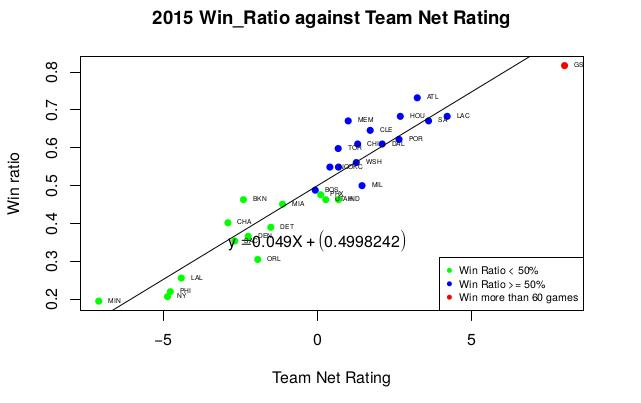
\includegraphics[width=\linewidth]{new_nr_15.jpg}
  \end{subfigure}
\bigskip

Figure 2: Comparison Between Net Rating and New Net Rating in 2015 Season
\end{figure}

\begin{figure}[h!]
  \centering
  \begin{subfigure}[b]{0.45\linewidth}
    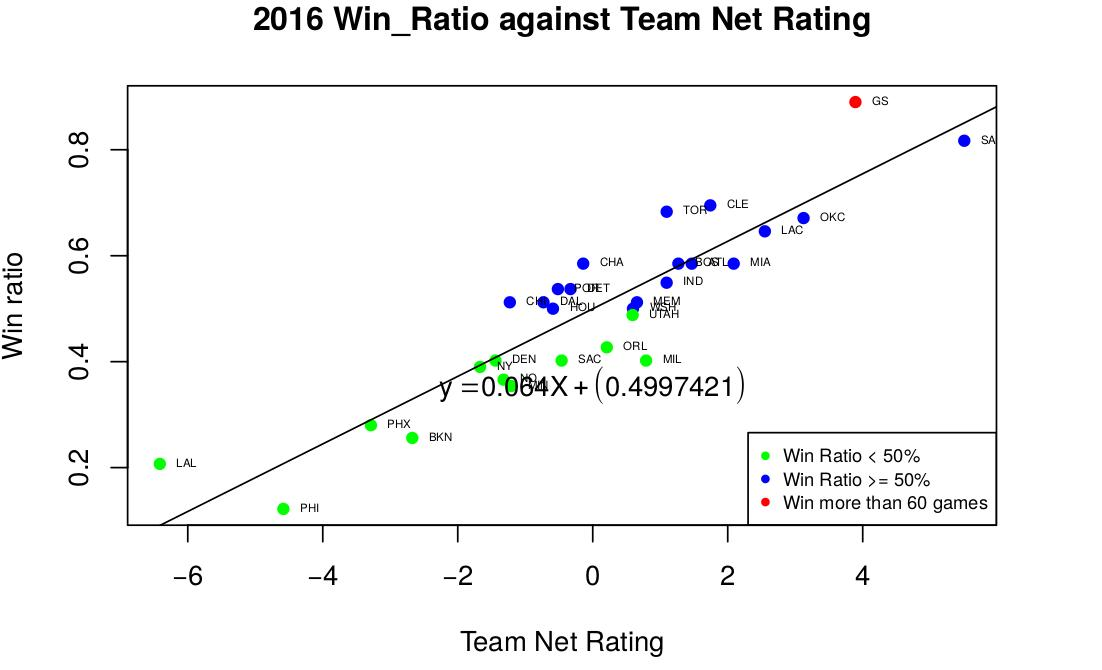
\includegraphics[width=\linewidth]{nr_16.jpg}
  \end{subfigure}
  \begin{subfigure}[b]{0.45\linewidth}
    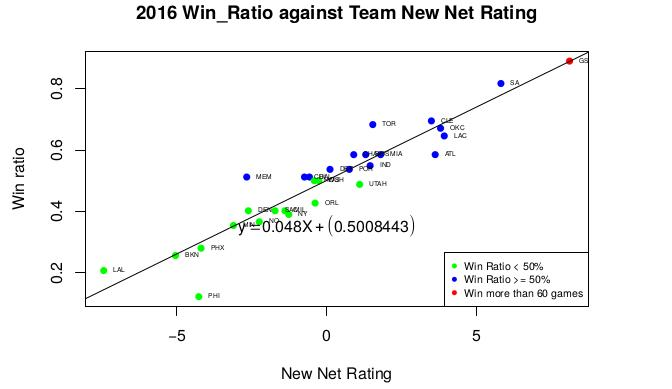
\includegraphics[width=\linewidth]{new_nr_16.jpg}
  \end{subfigure}


\bigskip

Figure 3: Comparison Between Net Rating and New Net Rating in 2016 Season
\end{figure}

\begin{figure}[h!]
  \centering
  \begin{subfigure}[b]{0.45\linewidth}
    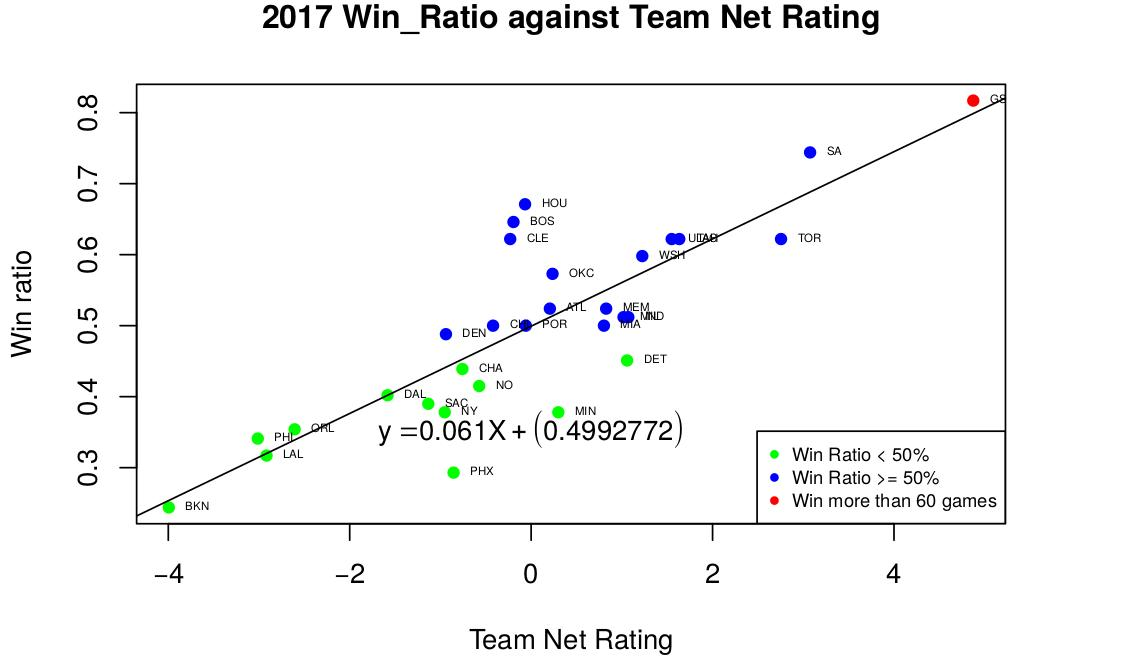
\includegraphics[width=\linewidth]{nr_17.jpg}
  \end{subfigure}
  \begin{subfigure}[b]{0.45\linewidth}
    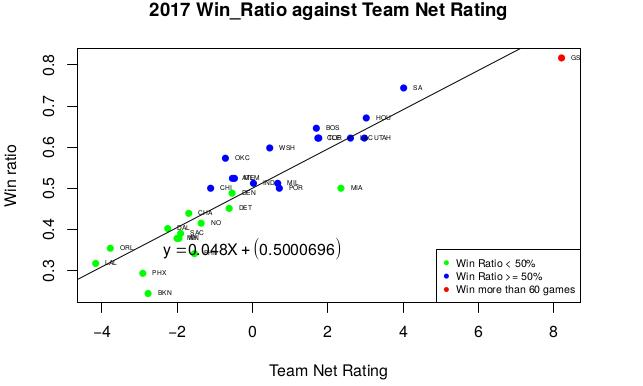
\includegraphics[width=\linewidth]{new_nr_17.jpg}
  \end{subfigure}

\bigskip

Figure 4: Comparison Between Net Rating and New Net Rating in 2017 Season
\end{figure}

\newpage
\subsubsection*{TOEs from 2014-2017 Seasons}
\begin{figure}[h!]
  \centering
  \begin{subfigure}[b]{0.45\linewidth}
    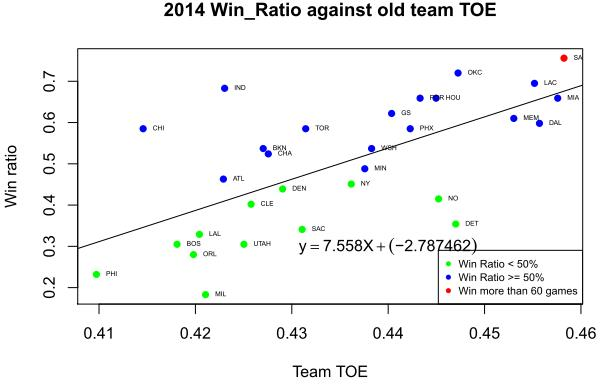
\includegraphics[width=\linewidth]{14old.jpg}
  \end{subfigure}
  \begin{subfigure}[b]{0.45\linewidth}
    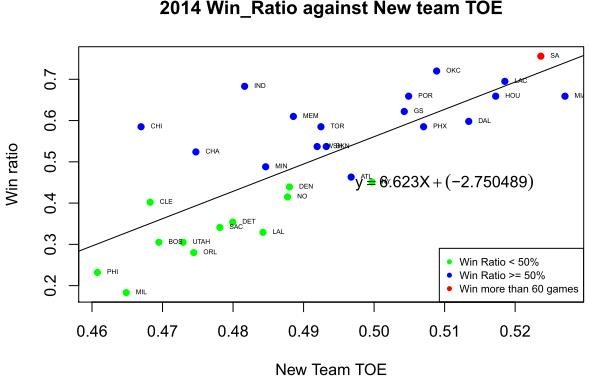
\includegraphics[width=\linewidth]{14new.jpg}
  \end{subfigure}
\bigskip

Figure 5: Comparision Between TOE and New TOE in 2014 Season

\end{figure}

\begin{figure}[h!]
  \centering
  \begin{subfigure}[b]{0.45\linewidth}
    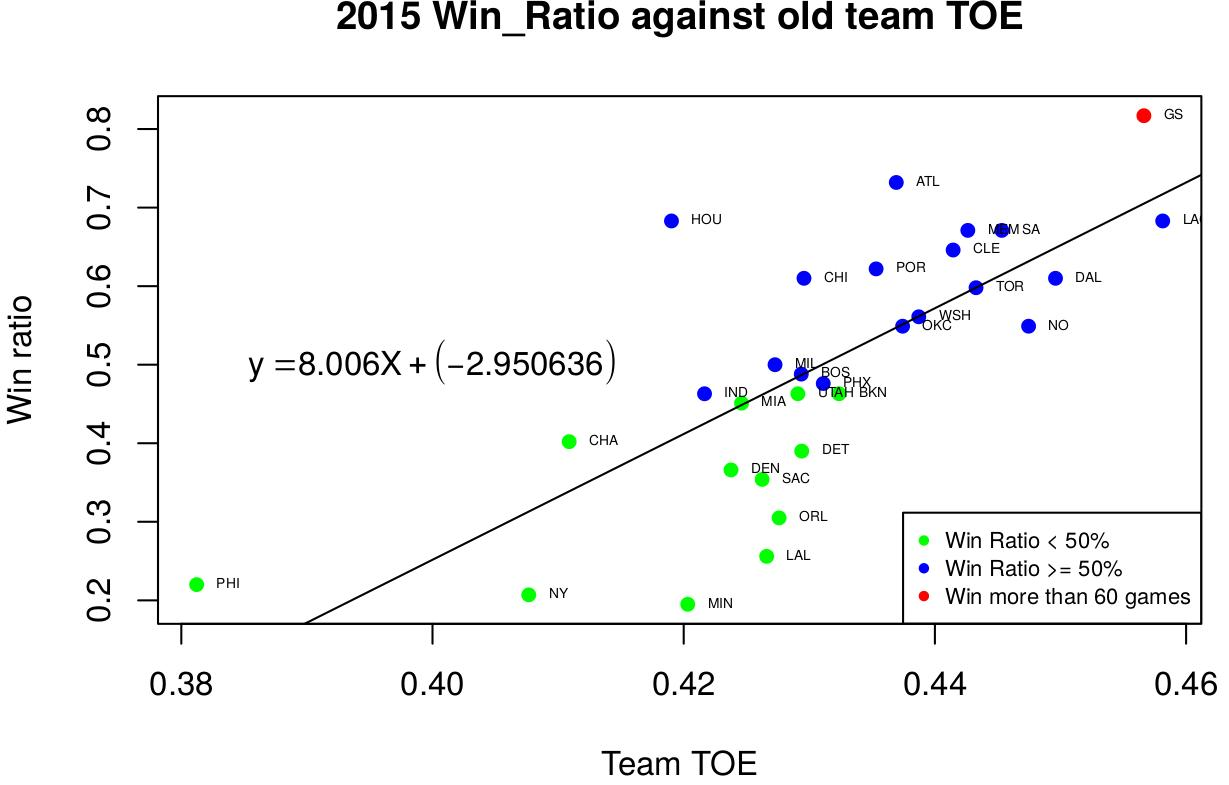
\includegraphics[width=\linewidth]{15old.jpg}
  \end{subfigure}
  \begin{subfigure}[b]{0.43\linewidth}
    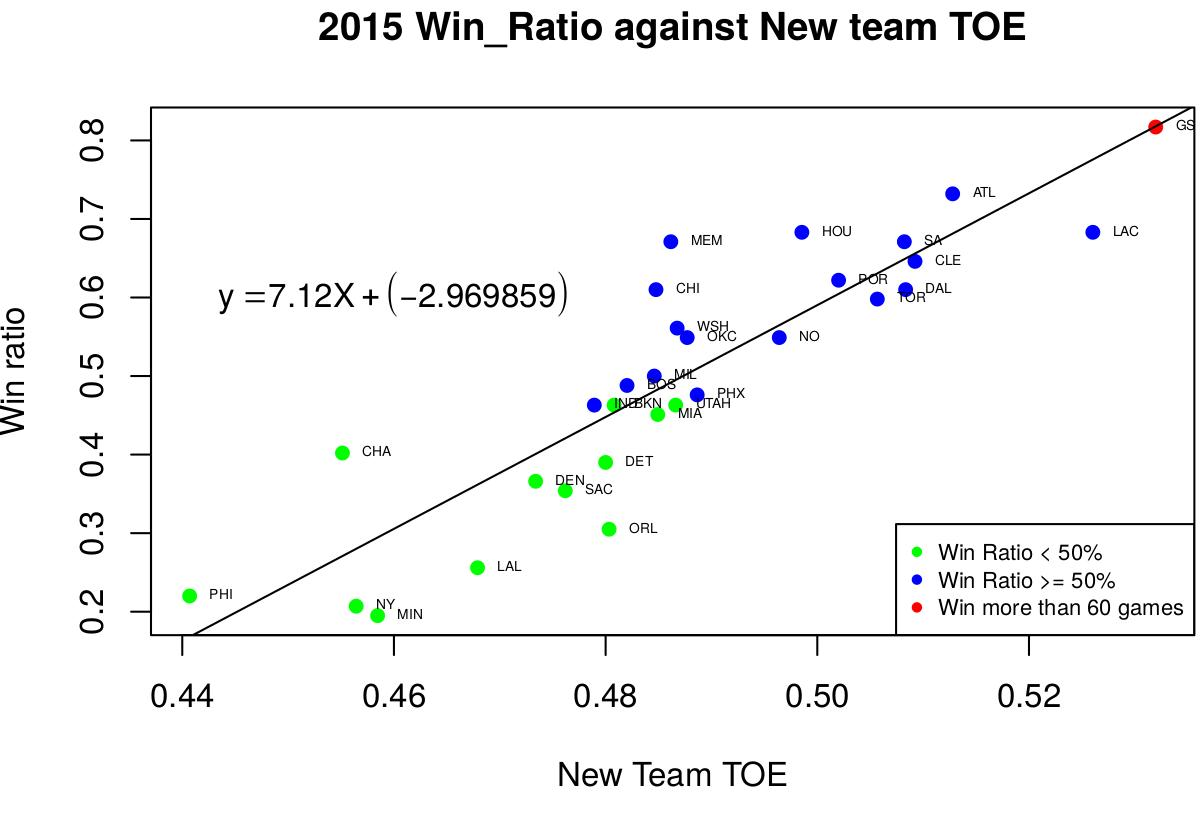
\includegraphics[width=\linewidth]{15new.jpg}
  \end{subfigure}
\bigskip

Figure 6: Comparision Between TOE and New TOE in 2015 Season
\end{figure}
\newpage	
\begin{figure}[h!]
  \centering
  \begin{subfigure}[b]{0.45\linewidth}
    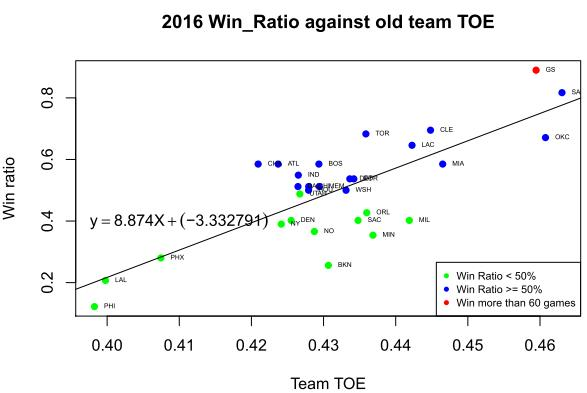
\includegraphics[width=\linewidth]{16old.jpg}
  \end{subfigure}
  \begin{subfigure}[b]{0.45\linewidth}
    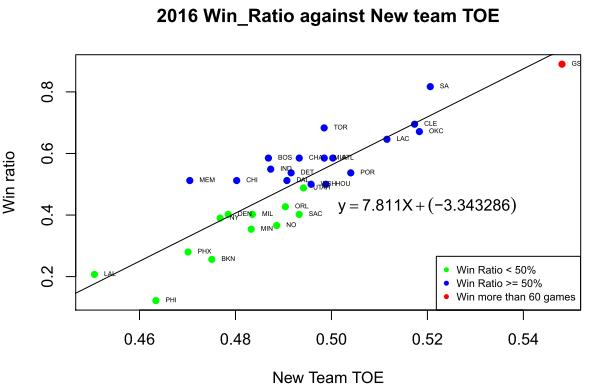
\includegraphics[width=\linewidth]{16new.jpg}
  \end{subfigure}
\bigskip

Figure 7: Comparision Between TOE and New TOE in 2016 Season
\end{figure}
\begin{figure}[h!]
  \centering
  \begin{subfigure}[b]{0.45\linewidth}
    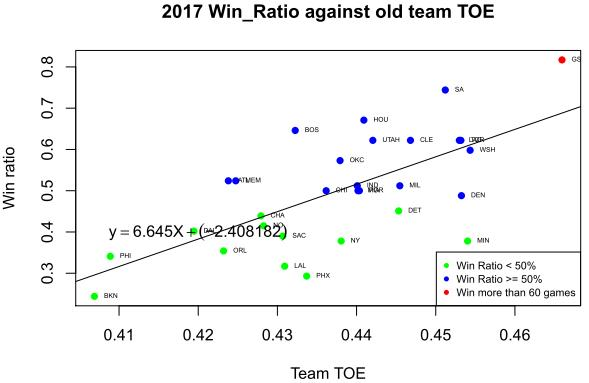
\includegraphics[width=\linewidth]{17old.jpg}
  \end{subfigure}
  \begin{subfigure}[b]{0.45\linewidth}
    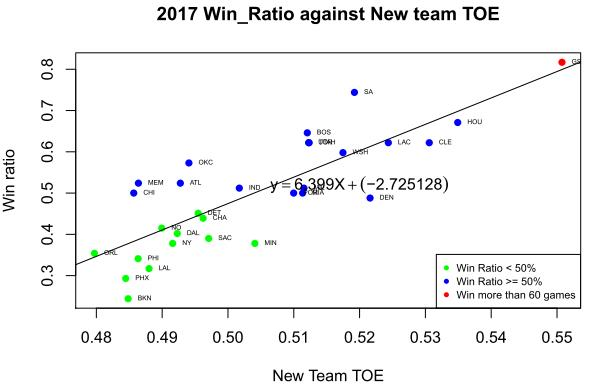
\includegraphics[width=\linewidth]{17new.jpg}
  \end{subfigure}
\bigskip

Figure 8: Comparision Between TOE and New TOE in 2017 Season
\end{figure}

\end{document}
